
\documentclass[paper=a4, fontsize=12pt]{scrartcl} 
\usepackage{amsmath,amsfonts,amsthm} % Math packages
\usepackage{graphicx}

\setlength{\parskip}{0.5em}


\numberwithin{equation}{section} % Number equations within sections (i.e. 1.1, 1.2, 2.1, 2.2 instead of 1, 2, 3, 4)
\numberwithin{figure}{section} % Number figures within sections (i.e. 1.1, 1.2, 2.1, 2.2 instead of 1, 2, 3, 4)
\numberwithin{table}{section} % Number tables within sections (i.e. 1.1, 1.2, 2.1, 2.2 instead of 1, 2, 3, 4)

\setlength\parindent{10pt} % Removes all indentation from paragraphs - comment this line for an assignment with lots of text

%----------------------------------------------------------------------------------------
%	TITLE SECTION
%----------------------------------------------------------------------------------------

\newcommand{\horrule}[1]{\rule{\linewidth}{#1}} % Create horizontal rule command with 1 argument of height

\title{	
\normalfont \normalsize 
\textsc{Chung-Ang University, Department of Computer Science and Engineering} \\ [25pt] % Your university, school and/or department name(s)
\horrule{0.5pt} \\[0.4cm] % Thin top horizontal rule
\huge Assignment 01 \\
Git Utility\\  % The assignment title
\horrule{1pt} \\[0.5cm] % Thick bottom horizontal rule
}

\author{Syed Farhan Alam Zaidi \\ (2018210031)} % Your name

\date{\normalsize\today} % Today's date or a custom date

\begin{document}

\maketitle % Print the title

%-----------------------------------------Body-----------------------------------

\section{Introduction to Git}
\par Git is a open source platform. It is available globally on git hub website and also in the form of desktop application with Graphical User Interface(GUI) for Windows, Mac and Linux platforms.  It is version control system that helps us to manage changes made to documents and other computer files. We can maintain source files, documentations, short stories, pictures and manage the large projects. Projects with lot of revision and changes can be backtracked to the older version. Multiple person can work at a time on the single project from different places.  The changes are clearly communicated with no error.

\section{How to use Git?}
\par For using the gitHub we have required GitHub account. We can sign-up account easily its free for every one. GitHub provides free unlimited storage publicly and chrages \$7 per month for private storage.  

   \par git config --global user.name "Syed Farhan Alam Zaidi"
   \par  git config --global user.email "syedfarhanalam1993@gmail.com"

\subsection{Create Repository}
\par After configure git, make directory with the command "mkdir assignment01", and enter in the working directory assignemnt01 using "cd assignment01". Than, initialize the repository with "git init" command. We can also do it by using GUI on website. see figure \ref{crepo}.

\begin{figure}
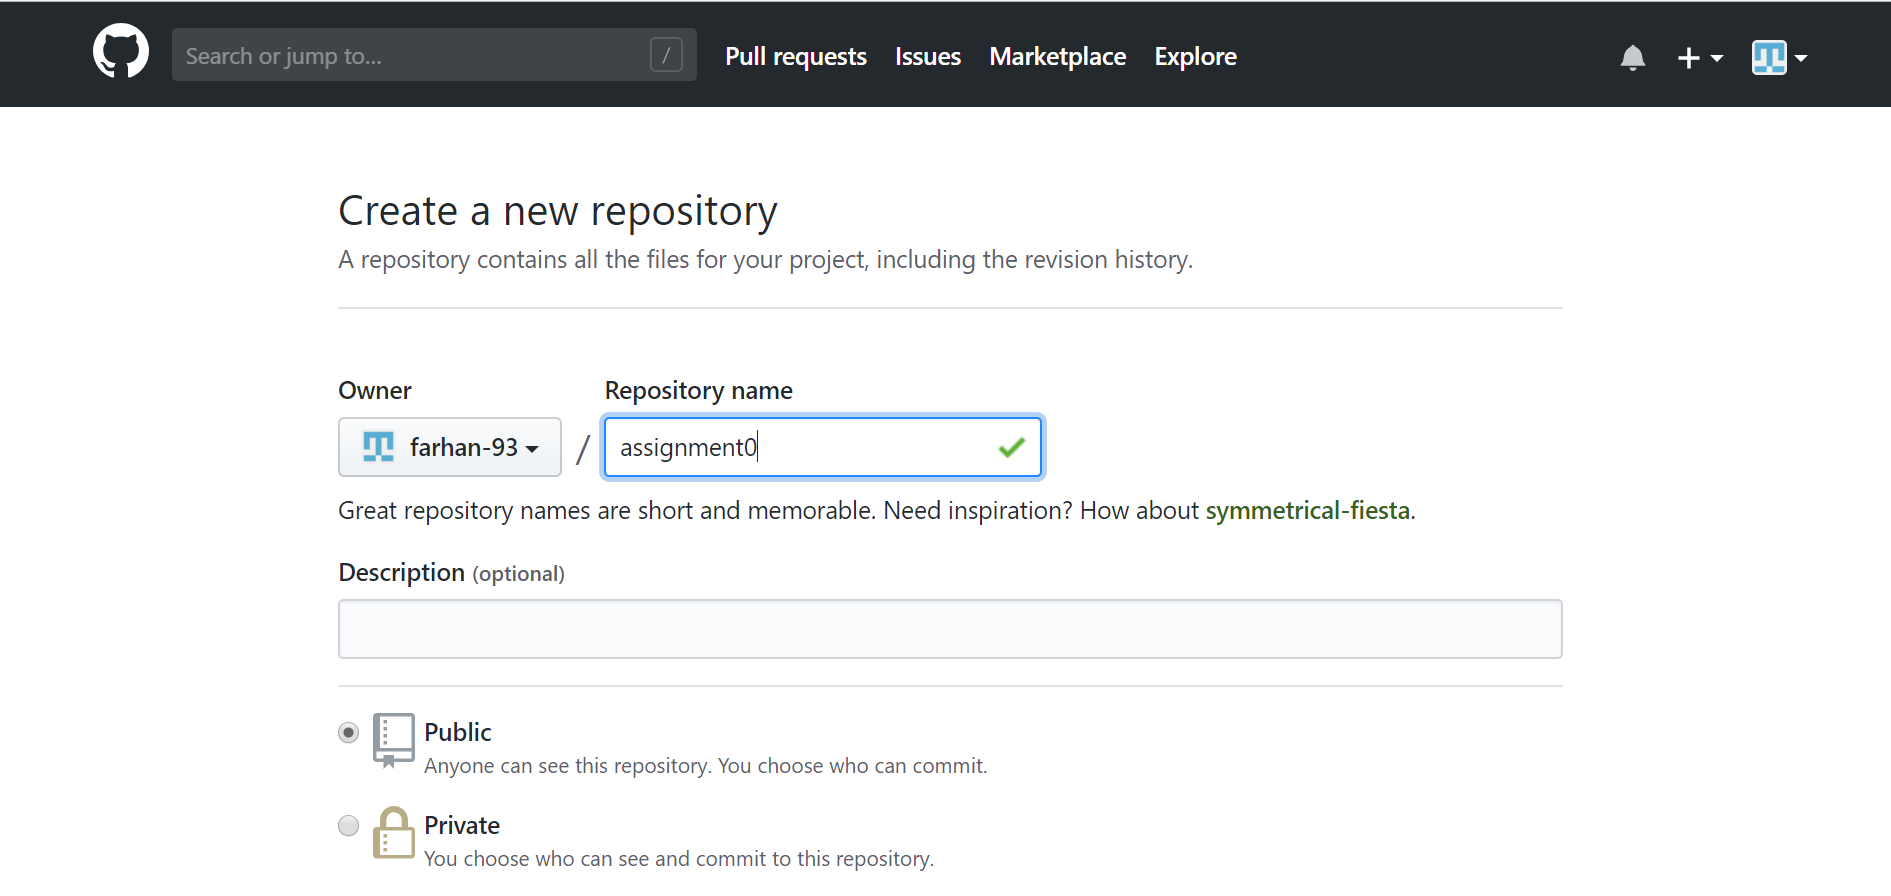
\includegraphics[width=\linewidth]{createrepository.PNG}
\caption{Create Repository}
\label{crepo}
\end{figure}

\subsection{Create file}
After create the repository I make a file. I created the file in assignment01 repository with the name "assignment01.tex" see figure \ref{cfile}.

\begin{figure}
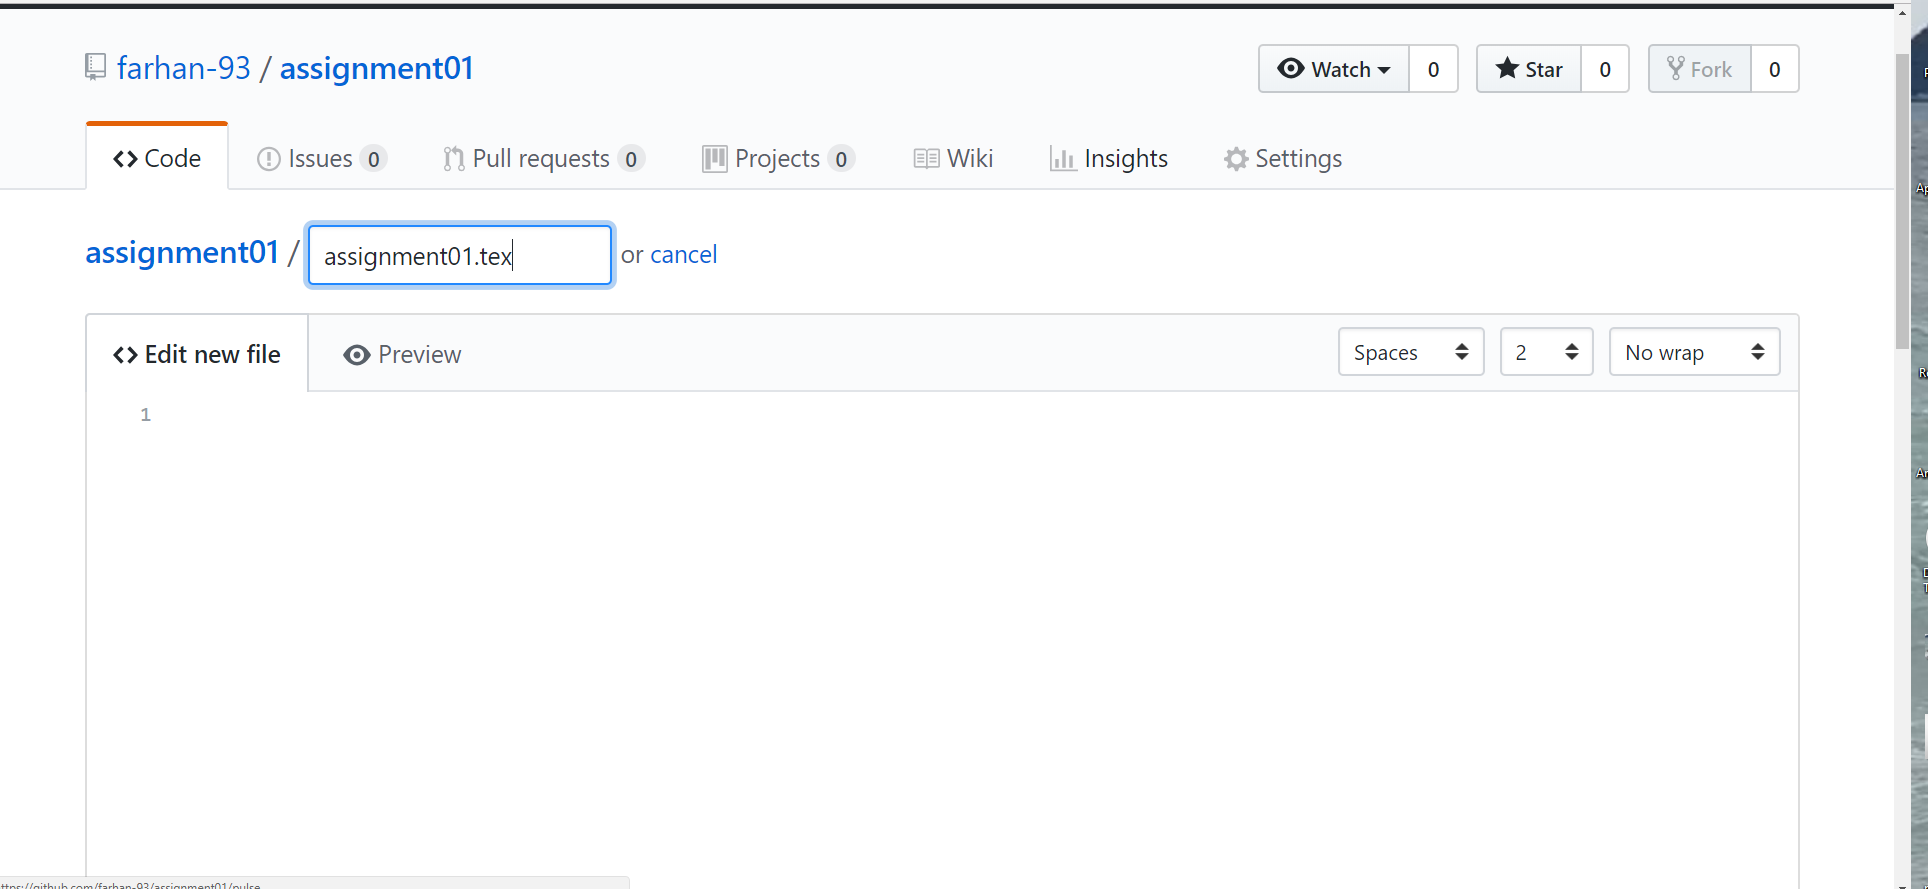
\includegraphics[width=\linewidth]{createfile.PNG}
\caption{Create file}
\label{cfile}
\end{figure}

\subsection{Commit}
Commit is the process of updating the repository. It saves the all updated files. After create the empty file, I modified the data in the .tex file. and than commit it. See figure \ref{ccom}.

\begin{figure}
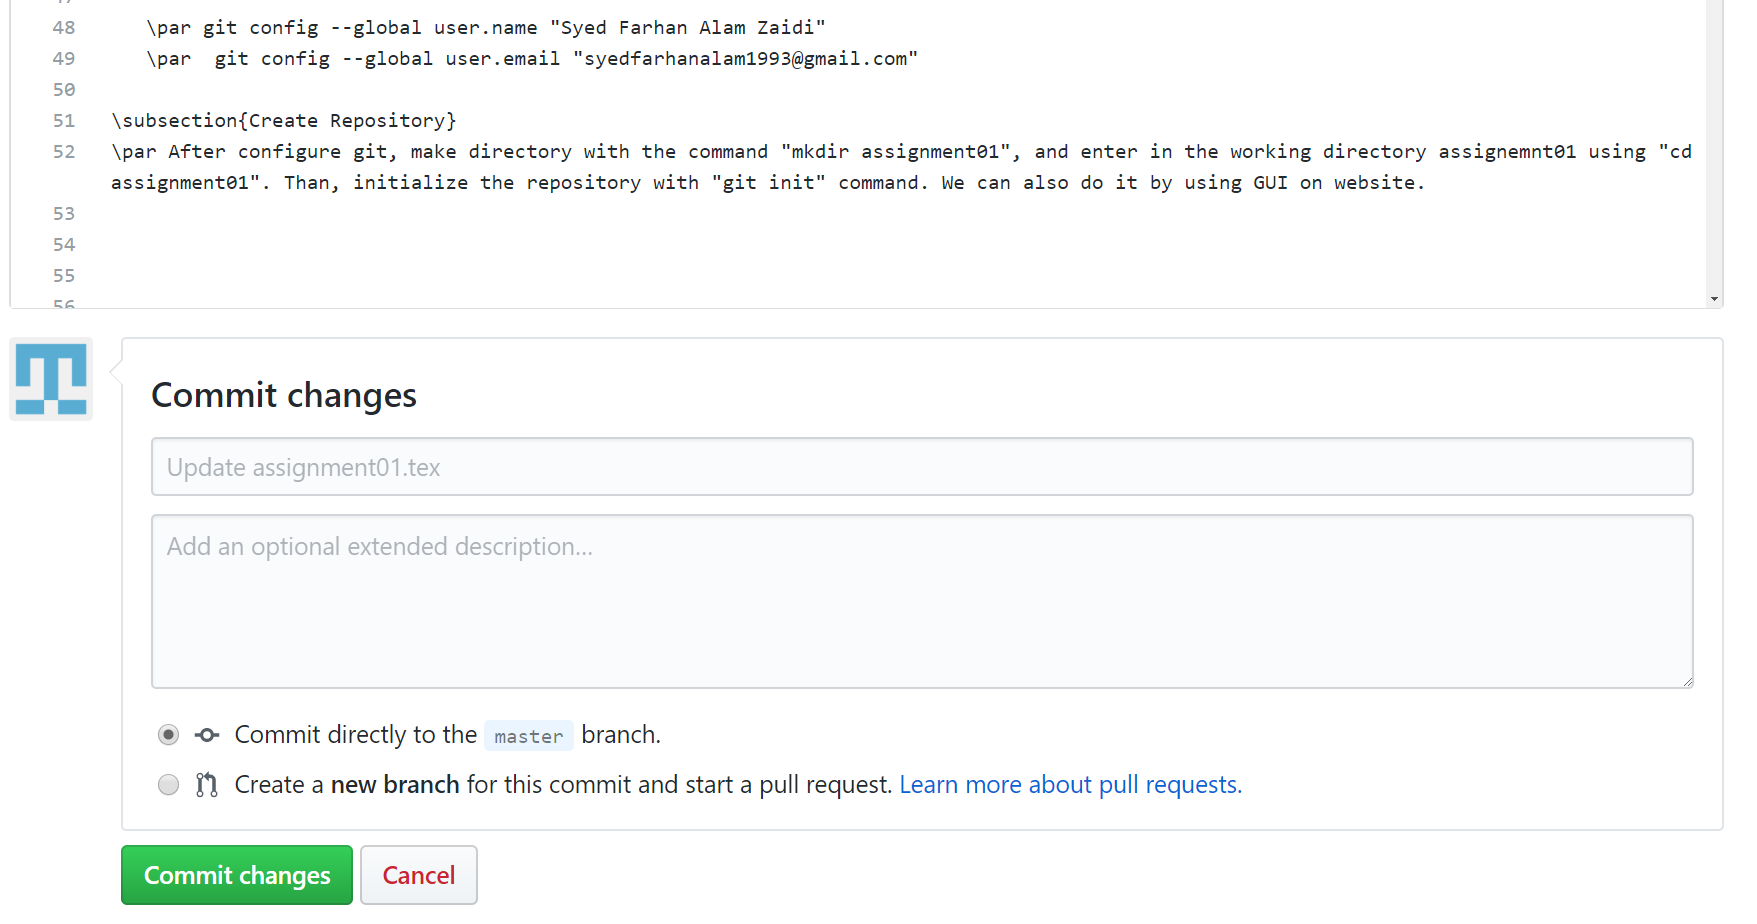
\includegraphics[width=\linewidth]{Commit.PNG}
\caption{Commit the file}
\label{ccom}
\end{figure}


\subsection{Pulling}
Pulling is the process of remotely access the file to the local computer. Local computer must has the git repository. 
The git repository can be create by \textit{"git init"} command. After creating the git repository on my local computer, pull the directory from gitHub. Shown in figure \ref{cpull}.



\begin{figure}
\includegraphics[width=\linewidth]{pull.png}
\caption{pull the file from "github.com/farhan-93/assignment01.git"}
\label{cpull}
\end{figure}




\subsection{Push}
Pushing is the process of remotely update the file to gitHub repository from the local computer. Local computer must has the git repository. The process of pushing is shown in figure \ref{cpush}.




\begin{figure}
\includegraphics[width=\linewidth]{pull.png}
\caption{push the file from local computer to "github.com/farhan-93/assignment01.git"}
\label{cpush}
\end{figure}


%----------------------------------------------------------------------------------------

\end{document}